\documentclass{article}

\usepackage[utf8]{inputenc}
\usepackage[english]{babel}
\usepackage{geometry}
\usepackage{setspace}
\usepackage{amsmath}
\usepackage{amssymb}

\usepackage{graphicx}
\graphicspath{{./images/}}

\usepackage{listings}
\lstset{
    language=Python,
    upquote=true,
    showstringspaces=false
    }
\usepackage{xcolor}

%New colors defined below
\definecolor{codegreen}{rgb}{0,0,0}
\definecolor{codegray}{rgb}{0,0,0}
\definecolor{codepurple}{rgb}{0,0,0}
\definecolor{backcolour}{rgb}{1,1,1}


%Code listing style named "mystyle"
\lstdefinestyle{mystyle}{
  backgroundcolor=\color{backcolour}, commentstyle=\color{codegreen},
  keywordstyle=\color{magenta},
  numberstyle=\tiny\color{codegray},
  stringstyle=\color{codepurple},
  basicstyle=\ttfamily\footnotesize,
  breakatwhitespace=false,         
  breaklines=true,                 
  captionpos=b,                    
  keepspaces=true,                 
  numbers=left,                    
  numbersep=5pt,                  
  showspaces=false,                
  showstringspaces=false,
  showtabs=false,                  
  tabsize=2
}

%"mystyle" code listing set
\lstset{style=mystyle}

\geometry{top=1in, bottom=1in, left=1in, right=1in}
\onehalfspacing

\title{SECLUSAL: A SupErvised CLUStering ALgorithm} 
\author{Yoshihiro Sato}
\date{February 2023}

\begin{document}

\begin{abstract}
A supervised clustering method that partitions data points into a limited number of clusters with respect to a target variable, based on the features specified by the user, is proposed.
The resulting clusters have the following characteristics: 
(i) The target variable has low variance within a cluster, but has high variance between clusters, and (ii) The data points in a cluster share similar values in the features that are relevant to distinguish the target. 
The method is robust to %the curse of dimensionality % YOSHI: this is a strong claim...
%as well as to 
the presence of irrelevant features and correlated features. 
This supervised clustering method also helps to increase the interpretability of machine learning models.
\end{abstract}

\maketitle

\section{Introduction}

Imagine you have a portfolio of customers you want to partition into several customer segments. Unsupervised clustering methods such as K-means and hierarchical clustering may be your first choice of methods. These are also what a standard machine learning textbook recommends you. 

There are some drawbacks in these methods. Firstly, there are a few technical issues. They aim to find centroids and classify data points that lay in the vicinity of each centroid. These methods presume that the distribution of data points in the feature space is uneven, so that you can find some dense areas. If the data points are distributed more or less evenly and continuously in the feature space, distinguishing one cluster from another becomes challenging. There is a risk that a small shift in the location of data points may change the clustering drastically.

The number of features used for clustering is another technical problem. In some cases, you may have a limited number of features available, but in many practical cases, there are too many potentially interesting features. For example, a customer relation management (CRM) system contains information on customers in different aspects. We often don’t know a priori which features are relevant for clustering. Using all those features to find centroids and their neighbors may easily end up with a problem -- the so-called curse of high dimensionality. 

We also need to remember that these standard clustering methods treat all input features as equally important. When the true underlying clusters present in the data differ only with respect to a small fraction of the features, other features included in the clustering may contaminate the result. When some of the features are correlated, then the dimension common in these features will be overrepresented in the clustering. Yet another limitation is that the method is not applicable when some of the features are non-numerical.

Thirdly, there is a practical concern. We usually have some target variables in mind when we apply clustering methods. For example, we may want to partition our customers with respect to the propensity to churn, or the likelihood to buy our products. Then, one of the goals of the clustering is to make the mean values of these target variables as distinctive as possible between the clusters. In some machine learning textbooks, the authors first introduce the K-means clustering method and apply it to data. They, then, compare the means of some target variable across the clusters to judge the performance of the clustering method. The performance is judged to be high if the target variable has distinct values between clusters. However, because the clustering method is unsupervised, the resulting clusters often fail to show high performance.

In this article, I propose a novel approach for supervised clustering. The approach I present here makes an active use of a target variable while clustering the data points based on the features you feed in. It has a number of advantages. The method generates a limited number of clusters that have the following characteristics: the target variable has low variance within a cluster, but has high variance between clusters. The data points in a cluster share similar values in the features. The method automatically selects the relevant features and only takes them into account during clustering. Thus, the method is robust to inclusion of irrelevant features as well as correlated features. Because the method does not need to measure the distance between data points, we don't suffer from the problems of high dimensionality.

\section{Idea}
My approach starts by applying the random forest algorithm to the (training) dataset. When you specify a target variable, the algorithm iteratively splits the data on the feature that results in the maximum gain in homogeneity with regards to the target. Each end node (leaf), then, contains the data points with similar values in the target. Besides, the data points in one end node also share similar values in the features that are relevant to predict the target. We repeatedly fit a decision tree to a random sample of the training set with replacement.

In the second step, we make a proximity matrix based on each fitted tree. This is a two-dimensional square matrix, where both rows and columns represent data points, and each cell represents a pair of data points. We assign 1 to the cell if the pair ends up in the same end node in the tree, and 0 otherwise. After making this proximity matrix for each tree, we take the average over the matrices. This is a final proximity matrix. To transform this matrix to a distance matrix, we subtract it from an all-ones matrix with the same shape. The resulting distance matrix shows the degree of the dissimilarity between each pair of the data points. (In the following illustrations, I only show the lower triangular elements of the proximity and distance matrices because they are symmetric matrices.)

In the third step, we apply the bottom-up hierarchical clustering method to this distance matrix.

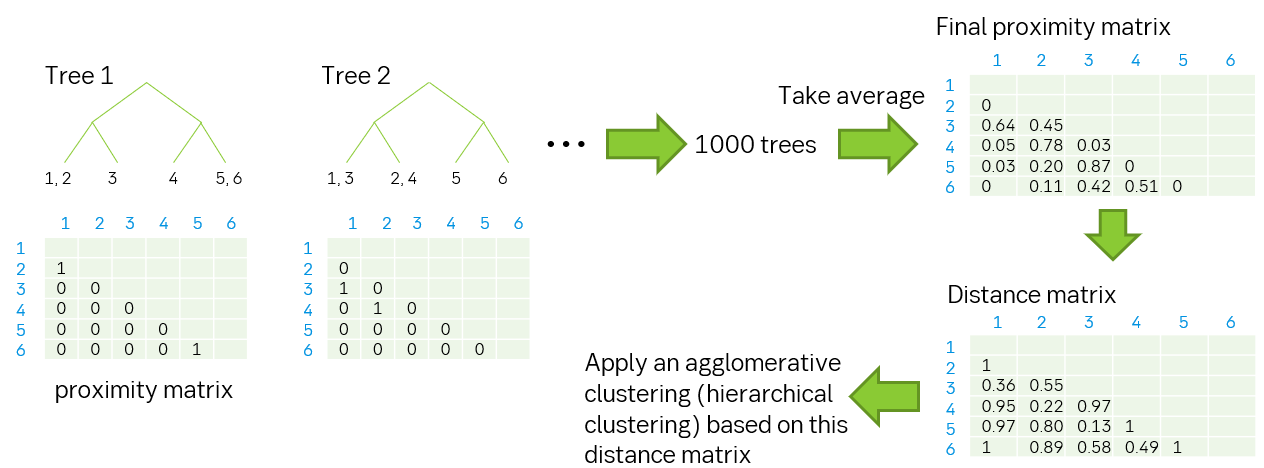
\includegraphics[width=1\textwidth]{supervised_clustering}

If we were only interested in partitioning data points with respect to a target variable, we could sort them in the target value and split them at some cut points. However, the algorithm I propose here takes into account both the target and features in making clusters. In a way, my approach can be seen as an attempt to define a block function $f:\mathbb{R}^n\rightarrow\mathbb{R}$.

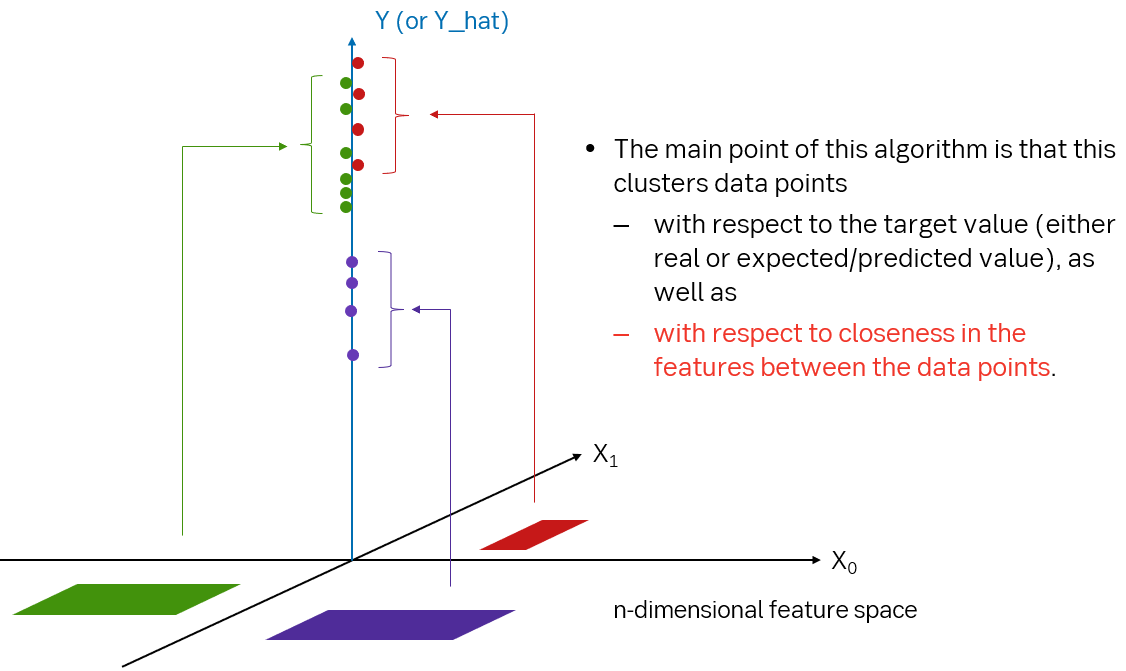
\includegraphics[width=1\textwidth]{block_function}

\section{Application to sample data}
\subsection{Data}
I explain my approach step-by-step using an example. I have a sample dataset of 4,000 customers. This is totally simulated data and not at all related to any real case. Assume that we are running an online shop for some products, and customers are required to join a membership program to buy the products. We have information on the customers who cancelled the membership and who retained the membership, as well as information on their characteristics and behaviors in the shop. The target is binary, taking 1 if the customer churned and 0 otherwise. 

The dataset can be found in the repo.

\begin{lstlisting}[language=Python]
X = pd.read_csv('./datasets/simulated_churn_example/X.csv')
y = pd.read_csv('./datasets/simulated_churn_example/y.csv')
print(X.shape)
print(y.shape)
\end{lstlisting}

\begin{lstlisting}[language=Python,numbers=none]
(4000, 8)
(4000, 1)
\end{lstlisting}

We have 8 features as follow:
\begin{itemize}
  \item \verb|age|: min = 20, median = 50.0, max = 79
  \item \verb|tenure| (membership period in months): min = 1, median = 34.5, max = 68
  \item \verb|n_monthly_visits| (number of online visits per month): min = 0, median = 5.0, max = 9
  \item \verb|monthly_charges| (amount of purchase per month): min = 5, median = 1471.0, max = 2994
  \item \verb|monthly_products| (number of purchased products per month): min = 1, median = 5, max = 16
  \item \verb|total_charges| (total amount of purchase): min = 25, median = 39135, max = 270102
  \item \verb|Irrelevant_1|: min = 0.0, median = 0.51, max = 1.0
  \item \verb|Irrelevant_2|: min = -3.26, median = 0.03, max = 2.91
\end{itemize}

Please observe that the last two features are just noise variables. The churn rate in this dataset is 21.5\%.

We want to split our customers into a limited number of clusters with respect to the propensity of churn. We also want the customers in each cluster to share similar values in the features related to the churn behavior. We don't know in advance which features are relevant for the clustering. We can imagine that some of the features are correlated to each other. The amount of purchase per month is likely to correlate with the number of purchased products per month. The total amount of purchases probably increases with the membership period.

I split the dataset into a training set (3,000 customers) and a test set (1,000 customers). The latter set will be used to check the performance of the clustering.

\begin{lstlisting}[language=Python]
from sklearn.model_selection import train_test_split
X_train, X_test, y_train, y_test = train_test_split(X, y, test_size=0.25, random_state=12)
print(X_train.shape)
print(X_test.shape)
print(y_train.shape)
print(y_test.shape)
\end{lstlisting}

\begin{lstlisting}[language=Python,numbers=none]
(3000, 8)
(1000, 8)
(3000, 1)
(1000, 1)
\end{lstlisting}

\subsection{Random forest}
I fit a random forest model with 1,000 trees to the training set. The max depth is set to 3. This is one of the important parameters that decide the granularity of the clusters. Regarding the choice of libraries to train random forest, you can choose whichever library you like. I choose LightGBM, but Skicit-learn and XGBoost can be alternatives.

\begin{lstlisting}[language=Python]
import lightgbm as lgb
    
lgb_data = lgb.Dataset(X_train, label=y_train, params={'feature_pre_filter': False})
params = {'boosting_type': 'rf',
          'objective': 'binary',
          'metric': 'binary',
          'max_depth': 3, 
          'min_child_samples': 1,
          'colsample_bytree': 0.5,
          'bagging_freq': 1,
          'bagging_fraction': 0.5,
          'n_jobs': 5,
          'random_state': 100,
          'verbose': -1}
rf = lgb.train(params, lgb_data,
               num_boost_round=1000,
               verbose_eval=-1)

y_train_pred = rf.predict(X_train)
print(classification_report(y_train, y_train_pred > 0.5))
\end{lstlisting}

\begin{lstlisting}[language=Python,numbers=none]
              precision    recall  f1-score   support

           0       0.94      0.97      0.95      2377
           1       0.86      0.76      0.81       623

    accuracy                           0.92      3000
   macro avg       0.90      0.86      0.88      3000
weighted avg       0.92      0.92      0.92      3000
\end{lstlisting}

\begin{lstlisting}[language=Python]
y_test_pred = rf.predict(X_test)
print(classification_report(y_test, y_test_pred > 0.5))
\end{lstlisting}

\begin{lstlisting}[language=Python,numbers=none]
              precision    recall  f1-score   support

           0       0.93      0.96      0.95       763
           1       0.86      0.77      0.82       237

    accuracy                           0.92      1000
   macro avg       0.90      0.87      0.88      1000
weighted avg       0.92      0.92      0.92      1000
\end{lstlisting}

\begin{lstlisting}[language=Python]
importance = pd.DataFrame(
    rf.feature_importance('gain'),
    index=X.columns, 
    columns=['importance(gain)']
).sort_values('importance(gain)', ascending=False)

importance['importance(gain)'] \
    = importance['importance(gain)'] / importance['importance(gain)'].sum()
print(importance)
\end{lstlisting}

\begin{lstlisting}[language=Python,numbers=none]
                  importance(gain)
age                       0.691407
monthly_charges           0.106510
monthly_products          0.102614
total_charges             0.045406
tenure                    0.028894
n_monthly_visits          0.021468
irrelevant_2              0.001936
irrelevant_1              0.001764
\end{lstlisting}

The performance of the trained model is fine. The predictions from both the training and test set have an overall accuracy of 0.92. The feature importance table shows that age is the most important feature, followed by monthly charges and monthly products.

\subsection{Proximity and distance matrices}

Let's construct a proximity matrix from the trained trees. In order to identify the customers in the training set that end up in the same end node, we need the node (leaf) id for each customer and for each tree. 

\begin{lstlisting}[language=Python]
pred_leaf = rf.predict(X_train, pred_leaf=True)
print(pred_leaf.shape)
\end{lstlisting}

\begin{lstlisting}[language=Python,numbers=none]
(3000, 1000)
\end{lstlisting}

\begin{lstlisting}[language=Python]
print(pred_leaf)
\end{lstlisting}

\begin{lstlisting}[language=Python,numbers=none]
[[6 6 2 ... 5 5 3]
 [6 6 2 ... 5 5 6]
 [5 1 1 ... 2 6 5]
 ...
 [2 2 2 ... 1 2 3]
 [6 6 2 ... 5 5 3]
 [6 6 2 ... 5 5 6]]
\end{lstlisting}

This is a $3,000$ (the number of customers in the training set) $\times$ $1,000$ (the number of trees) matrix. A column contains the end node (leaf) id of each customer in a tree.

Converting this node id matrix to a proximity matrix is time-- and memory--consuming. Because a proximity matrix from a single tree is symmetric and most of the cells will be filled with zeros, I first define the function \verb|proximity_matrix_tril_from_single_array| that generates a sparse lower triangular matrix from a column in the node id matrix. This function is, then, applied to all trees by loop and the average values are taken over the trees by the function \verb|proximity_matrix_tril_loop|. Finally, the sparse lower triangular matrix is converted to a dense proximity matrix through the function \verb|to_dense_proximity_matrix|.

\begin{lstlisting}[language=Python]
from scipy.sparse import csr_matrix, tril

def proximity_matrix_tril_from_single_array(array):
    """
    Convert an array of leaf ids from a single decision tree in random forest to a proximity matrix.
    Return it as a lower triangle matrix (because the matrix is symmetric. This is to reduce the memory use).
    """
    rval = np.zeros((len(array), len(array)), dtype=np.uint16)
    for leaf in np.unique(array):
        rval[array == leaf] = (array == leaf)
    return tril(rval, k=-1)

def proximity_matrix_tril_loop(pred_leaf):
    """
    Apply 'proximity_matrix_tril_from_single_array' to all trees by loop.
    This does not require as much memory as the functional counterpart, but takes longer time to complete.
    Then, take the average over the trees.
    
    pred_leaf: a matrix (2d-array) with n_observations * n_trees
    """
    for i in range(pred_leaf.shape[1]):
        if i % 10 == 0:
            print(i)

        array = pred_leaf[:, i]
        proximity_matrix_tril = proximity_matrix_tril_from_single_array(array)
        if i == 0:
            sum_proximity_matrix_tril = proximity_matrix_tril
        else:
            sum_proximity_matrix_tril += proximity_matrix_tril
            
    proximity_mtx_tril = (sum_proximity_matrix_tril/pred_leaf.shape[1]).astype(np.float16)
    return proximity_mtx_tril

def to_dense_proximity_matrix(proximity_matrix_tril):
    """
    Convert a lower triangle proximity matrix to a dense matrix.
    """
    result = proximity_matrix_tril \
        + proximity_matrix_tril.T \
        + np.eye(proximity_matrix_tril.shape[0], dtype=np.float16)
    return result
\end{lstlisting}

\begin{lstlisting}[language=Python]
proximity_mtx_tril = proximity_matrix_tril_loop(pred_leaf) # a lower triangle matrix
proximity_mtx = to_dense_proximity_matrix(proximity_mtx_tril) # a dense matrix
print(proximity_mtx.shape)
\end{lstlisting}

\begin{lstlisting}[language=Python,numbers=none]
(3000, 3000)
\end{lstlisting}

\begin{lstlisting}[language=Python]
print(proximity_mtx[:6, :6])
\end{lstlisting}

\begin{lstlisting}[language=Python,numbers=none]
[[1.         0.83496094 0.02999878 0.09002686 0.80615234 0.15698242]
 [0.83496094 1.         0.03799438 0.11199951 0.94384766 0.27392578]
 [0.02999878 0.03799438 1.         0.30297852 0.02799988 0.01699829]
 [0.09002686 0.11199951 0.30297852 1.         0.10797119 0.06799316]
 [0.80615234 0.94384766 0.02799988 0.10797119 1.         0.23803711]
 [0.15698242 0.27392578 0.01699829 0.06799316 0.23803711 1.        ]]
\end{lstlisting}

The resulting dense proximity matrix is a square symmetric matrix of $3,000 \times 3,000$ (the number of customers in the training set). This proximity matrix is converted to a distance matrix by subtracting each element from one. In order to enlarge the variance of the distance, I take the square of each element, which is just optional.

\begin{lstlisting}[language=Python]
# distance_mtx = 1 - proximity_mtx
# To enlarge the variance of the distance, it is squared.
distance_mtx = np.square(1 - proximity_mtx)
print(distance_mtx[:6, :6])
\end{lstlisting}

\begin{lstlisting}[language=Python,numbers=none]
[[0.         0.02723789 0.94090235 0.82805115 0.03757691 0.71067864]
 [0.02723789 0.         0.9254548  0.7885449  0.00315309 0.5271838 ]
 [0.94090235 0.9254548  0.         0.48583895 0.9447842  0.9662924 ]
 [0.82805115 0.7885449  0.48583895 0.         0.7957154  0.8686367 ]
 [0.03757691 0.00315309 0.9447842  0.7957154  0.         0.58058745]
 [0.71067864 0.5271838  0.9662924  0.8686367  0.58058745 0.        ]]
\end{lstlisting}

\subsection{Agglomerative clustering based on the distance matrix}

This distance matrix is fed into the agglomerative cluster function in the Scikit learn package, which generates a linkage matrix. Based on the linkage matrix, the dendrogram function from the Scipy package draws a hierarchical clustering tree. 

\begin{lstlisting}[language=Python]
from sklearn.cluster import AgglomerativeClustering
from scipy.cluster.hierarchy import dendrogram

def compute_linkage(model):
    """
    Create linkage matrix for plotting the dendrogram
    """

    # create the counts of samples under each node
    counts = np.zeros(model.children_.shape[0])
    n_samples = len(model.labels_)
    for i, merge in enumerate(model.children_):
        current_count = 0
        for child_idx in merge:
            if child_idx < n_samples:
                current_count += 1  # leaf node
            else:
                current_count += counts[child_idx - n_samples]
        counts[i] = current_count

    linkage_matrix = np.column_stack([model.children_, model.distances_,
                                      counts]).astype(float)
    return linkage_matrix
\end{lstlisting}

\begin{lstlisting}[language=Python]
ac = AgglomerativeClustering(
    distance_threshold=0, 
    n_clusters=None, 
    affinity='precomputed', 
    compute_full_tree=True, 
    compute_distances=True, linkage='average')
ac.fit_predict(np.asarray(distance_mtx))
linkage = compute_linkage(ac)

fig, ax = plt.subplots(figsize=(10, 5)) 
plt.title('Hierarchical Clustering Dendrogram')
dendrogram(linkage, ax=ax)
plt.show()
\end{lstlisting}

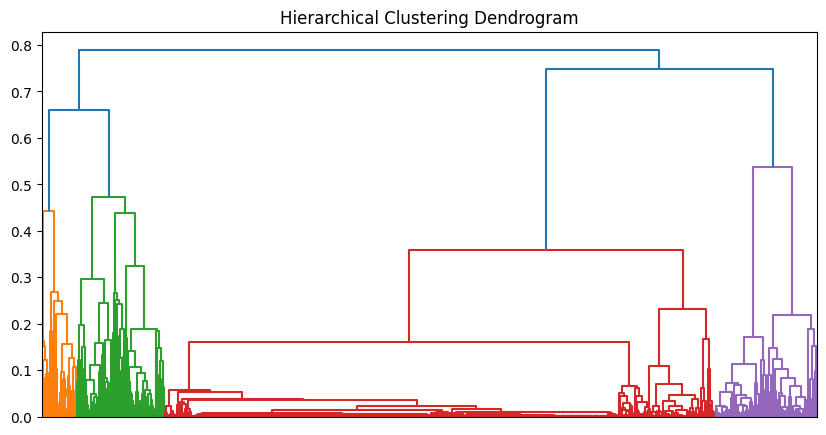
\includegraphics[width=1\textwidth]{dendrogram_depth3}

Nodes, or leaves, represent 3,000 customers in the training set. The four colors here are automatically chosen by the dendrogram function. The drawn tree suggests that we will get four clusters if we cut the tree at the distance of 0.6.

Instead of using the pre-determined distinctive colors, the function \verb|plot_colored_dendrogram| below colors each branch according to the average of the churn probability predicted by the random forest model from the end nodes up to the branch.

\begin{lstlisting}[language=Python]
from matplotlib import cm
from matplotlib.cm import get_cmap
from matplotlib.colors import to_hex
from matplotlib.colors import Normalize

def get_root_items(linkage):
    """
    A function used in 'get_item_average' to color dendrogram.
    """
    
    dict_items = {}
    for i, (item1, item2) in enumerate(linkage[:, :2].astype(int)):
        lst = []
        for item in [item1, item2]:
            if dict_items.get(item):
                lst += dict_items[item]
            else:
                lst.append(item)
        lst.sort()
        dict_items[i + len(linkage) + 1] = lst
    return dict_items

def get_item_average(linkage, y):
    """
    Compute the average value of 'y' under each (non-end) node.
    """
    
    dict_items = get_root_items(linkage)
        
    dict_y = {key: np.mean(y[value]) for key, value in dict_items.items()}
    return dict_y

def plot_colored_dendrogram(ac_model, clusters, y, cmap='jet', **kwargs):
    linkage = compute_linkage(ac_model)
    dict_items = get_root_items(linkage)
    if isinstance(y, pd.core.series.Series) or isinstance(y, pd.core.frame.DataFrame):
        y = y.values
    
    linkage_new = np.hstack([np.array(range(len(linkage)+1, len(linkage)*2+1)).reshape(-1, 1), linkage])
    n_clusters = len(np.unique(clusters))
    roots = [int(linkage_new[-1, 0])]
    for i in range(1, n_clusters):
        remove = int(linkage_new[-i, 0])
        add = [int(linkage_new[-i, 1]), int(linkage_new[-i, 2])]
        roots.remove(remove)
        roots += add # "roots" is a list of the root for each cluster
        
    dict_roots = {}
    for root in roots:
        if root < len(linkage):
            dict_roots[root] = clusters[root]
        else:
            dict_roots[root] = clusters[dict_items[root][0]]
    labels = [dict_roots.get(x) for x in range(len(linkage)+1, len(linkage)*2+1)]
    
    item_average = get_item_average(linkage, y)
    
    cmap = get_cmap(cmap)
    norm = Normalize(vmin=np.min(y), vmax=np.max(y))
    dn = dendrogram(linkage, link_color_func=lambda x: to_hex(cmap(norm(item_average[x]))), **kwargs)
    ii = np.argsort(np.array(dn['dcoord'])[:, 1])
    for j, (icoord, dcoord) in enumerate(zip(dn['icoord'], dn['dcoord'])):
        x_coord = 0.5 * sum(icoord[1:3])
        y_coord = dcoord[1]
        ind = np.nonzero(ii == j)[0][0]
        ax.annotate(labels[ind], (x_coord, y_coord), va='top', ha='center', fontsize=18, color='red')
\end{lstlisting}

\begin{lstlisting}[language=Python]
ac = AgglomerativeClustering(
    distance_threshold=0.45, 
    n_clusters=None, 
    affinity='precomputed',
    compute_full_tree=True, 
    compute_distances=True, 
    linkage='average')
clusters = ac.fit_predict(np.asarray(distance_mtx))

# The dendrogram is colorred according to the expected y values, averaged at each node.
fig, ax = plt.subplots(figsize=(12, 6)) 
plt.title('Hierarchical Clustering Dendrogram')
plot_colored_dendrogram(ac, clusters, y_train_pred, labels=['']*distance_mtx.shape[0])
plt.show()
\end{lstlisting}

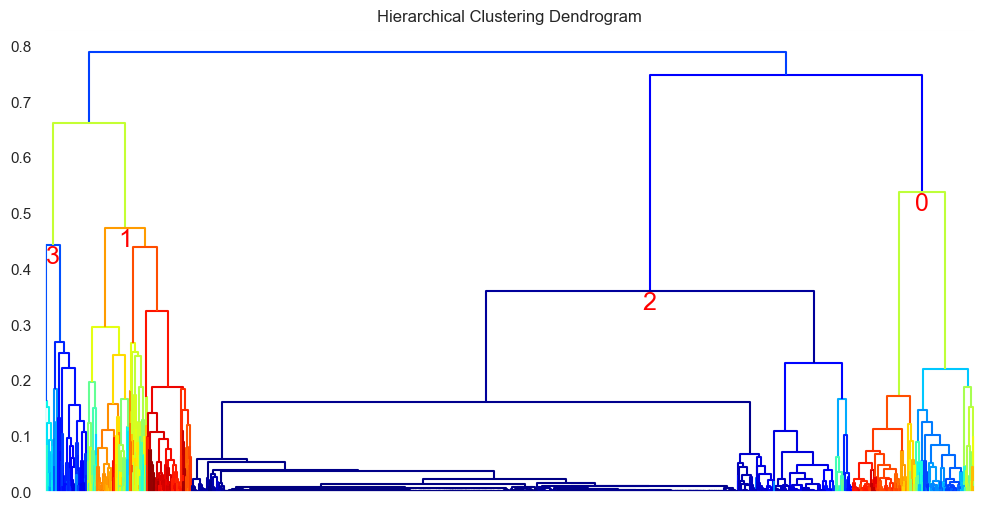
\includegraphics[width=1\textwidth]{dendrogram_depth3_colored_thres060}

The four clusters are marked with the cluster id in red, from 0 to 3. As already mentioned, the color represents the average of the predicted churn probability of the data points (end points) included in the branch. Blue indicates that the churn probability is predicted to be low while the red color indicates a high predicted churn probability. You see that Cluster 2 is the largest in the number of customers, and the churn probability of these customers is expected to be low. Cluster 3 is also made up of customers with a low expected churn probability, but those customers constitute a different subset. Clusters 0 and 1, on the other hand, cover customers who are expected to have a high churn probability. 

The table below shows the number of customers (\verb|count|) and its relative size (\verb|proportion|), as well as the averages of the actual binary target (\verb|target(y)|) and predicted churn probabilities (\verb|target(y_hat)|), by cluster. As we expect from the colors of the branches in the dendrogram, there is a large difference in these averages between clusters.

\begin{lstlisting}[language=Python]
def compute_target_mean_by_cluster(X, features, clusters, y, y_hat=None):
    df_cluster = pd.DataFrame(X, columns=features).copy()
    if isinstance(y, pd.core.series.Series) or isinstance(y, pd.core.frame.DataFrame):
        y = y.values
    df_cluster['y'] = y
    if y_hat is not None:
        df_cluster['y_hat'] = y_hat
    df_cluster['cluster_id'] = clusters
    mean_by_cluster_y = df_cluster.groupby('cluster_id')['y'].agg(['count', 'mean'])
    mean_by_cluster_y.columns = ['count', 'target(y)']
    if y_hat is not None:
        mean_by_cluster_y_hat = df_cluster.groupby('cluster_id')['y_hat'].agg(['mean'])
        mean_by_cluster_y_hat.columns = ['target(y_hat)']
    if y_hat is not None:
        df_rval = pd.concat([mean_by_cluster_y, mean_by_cluster_y_hat], axis=1)
    else:
        df_rval = mean_by_cluster_y
    df_rval['proportion'] = df_rval['count'] / df_rval['count'].sum()
    df_rval = df_rval.sort_index()
    if y_hat is not None:
        return df_rval[['count', 'proportion', 'target(y)', 'target(y_hat)']]
    return df_rval[['count', 'proportion', 'target(y)']]

per_cluster = compute_target_mean_by_cluster(X_train, X.columns, clusters, y_train, y_train_pred)
print(per_cluster)
\end{lstlisting}

\begin{lstlisting}[language=Python,numbers=none]
            count  proportion  target(y)  target(y_hat)
cluster_id                                             
0             392    0.130667   0.599490       0.583819
1             339    0.113000   0.787611       0.723926
2            2132    0.710667   0.050188       0.115921
3             137    0.045667   0.102190       0.265285
\end{lstlisting}

Let’s analyze the distribution of customers in the feature space by cluster. The box plots below show the distribution of feature values by cluster and by feature. The box width represents the relative size of the cluster and the box color explains the average value of the expected churn probability. Again, blue indicates a low churn probability whereas red indicates a high churn probability. Except for the last three features, there are more or less distinct distributions of features between clusters. Note the distinctiveness is strongly related to the feature importance obtained from the random forest model as we saw before. 

\begin{lstlisting}[language=Python]
pd_cluster = pd.DataFrame(X_train, columns=X.columns).copy()
pd_cluster['y_hat'] = y_train_pred
pd_cluster['y'] = y_train
pd_cluster['cluster_id'] = clusters

sns.set()
colors = per_cluster['target(y_hat)'].values
cmap = get_cmap('bwr')
norm = Normalize(vmin=np.min(colors), vmax=np.max(colors))
colors = [to_hex(x) for x in cmap(norm(colors))]

max_width = 0.9
min_width = 0.1
widths = per_cluster['proportion'].values
widths = (max_width - min_width) * widths / widths.max() + min_width

fig, ax = plt.subplots(4, 2, figsize=(12, 14))
    
for i, axi in enumerate(ax.flat):
    feature = importance.index[i]
    bins, groups = zip(*pd_cluster.groupby('cluster_id')[feature])
    bplot = axi.boxplot(groups, widths=widths, patch_artist=True, 
                showfliers=False, 
                medianprops=dict(color="white", linewidth=1.5))
    axi.set_xticklabels(bins)
    axi.set_ylabel(feature)
    axi.set_xlabel('cluster')
    
    for box, color in zip(bplot['boxes'], colors):
        box.set_facecolor(color)
    plt.colorbar(cm.ScalarMappable(norm=norm, cmap=cmap), ax=axi)
plt.show()
\end{lstlisting}

\begin{center}
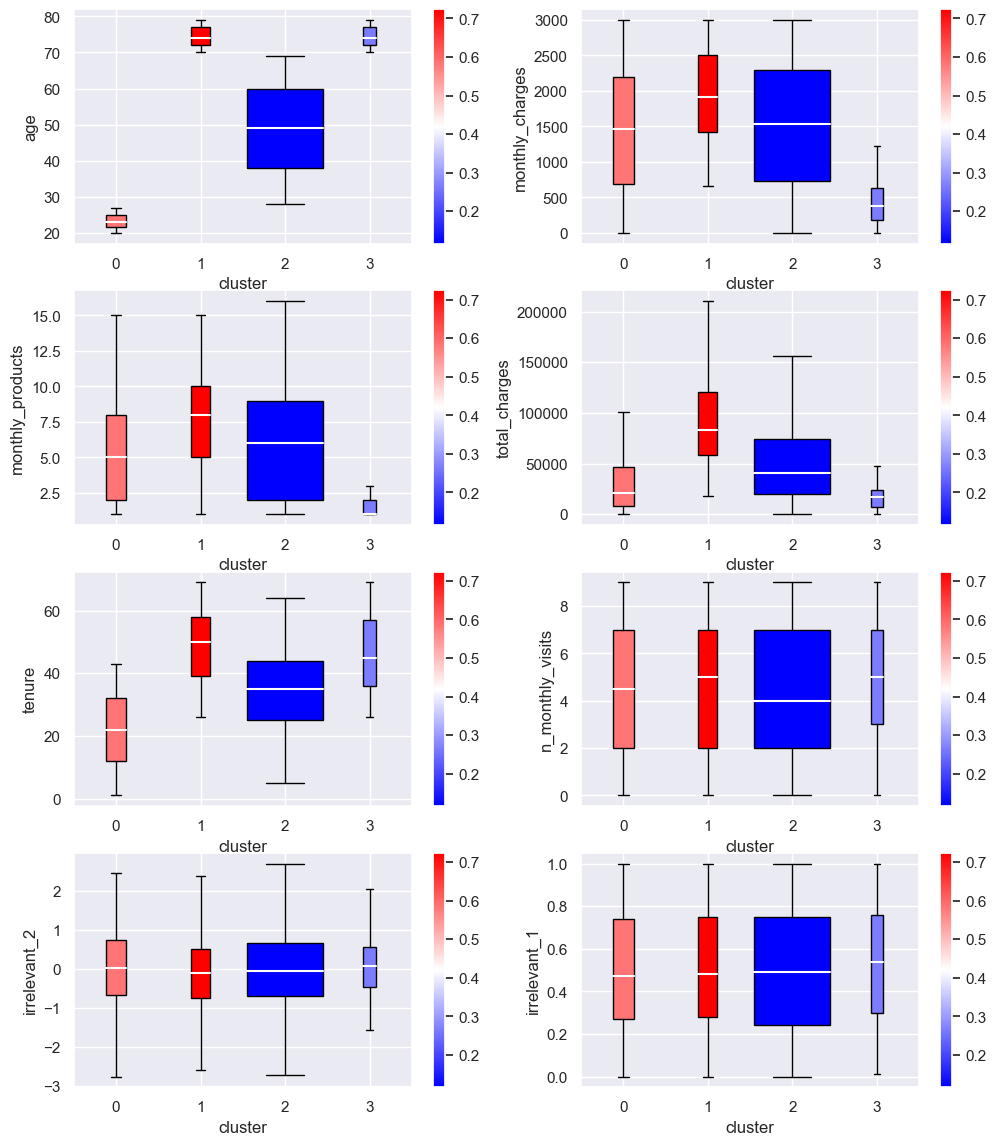
\includegraphics[width=1\textwidth]{dendrogram_depth3_thres060_features}
\end{center}

\subsection{Customer profiling}
The profile of each cluster can be summarized in the following table.

\begin{center}
\begin{tabular}{ |c||c c c c| } 
\hline
& cluster 0 & cluster 1 & cluster 2 & cluster 3 \\ 
\hline
Age & Young & Old & Middle & Old \\ 
Monthly charges & Middle & Middle-Large & Middle & Small\\ 
Monthly products & Middle & Middle-Many & Middle & Few\\ 
Total charges & Small & Large & Middle & Small\\ 
Tenure & Short & Long & Middle & Long \\ 
\hline \hline
Churn probability & High & High & Low & Middle\\ 
\hline
\end{tabular}
\end{center}

An interesting fact is revealed by this analysis: likely-to-churn customers are not a homogenous group, but they are rather split in two groups: Young customers with short tenure who purchase moderately (Cluster 0) and old customers with long tenure who purchase intensively (Cluster 1). The analysis here reveals the factors that determine the level of churn probability.

This implies, in fact, that this supervised clustering method is not only useful in clustering the data points, but also in helping us interpret machine learning models that tend to be black boxes. To a question, such as, ``What kind of customers tend to have a high churn probability?'', you can answer as follows: ``The customer of young age who has a short period as a customer and has spent little so far in total, or the customer of old age who has a long period as a customer and has spent a lot in total'', for example.

\subsection{Clustering of new data}
Even if we are successful in partitioning customers both in terms of the target variable and feature variables, how shall we apply this clustering model to new incoming data? In this section, I will show you how to apply the supervised clustering model trained on the existing customers to new, unseen customers.

All we need is to train a decision tree on the training set using the obtained cluster ids as a target.

\begin{lstlisting}[language=Python]
from sklearn.tree import DecisionTreeClassifier, export_graphviz
from pydotplus import graph_from_dot_data
from sklearn.metrics import confusion_matrix
import graphviz

tree = DecisionTreeClassifier(criterion='entropy', max_depth=3, random_state=1)
tree.fit(X_train, clusters)

print(tree.score(X_train, clusters))
\end{lstlisting}

\begin{lstlisting}[language=Python,numbers=none]
0.99567
\end{lstlisting}

This trained tree fits the training set very well: it predicts the cluster id almost perfectly. The confusion matrix below shows there are only a few misclassifications. 

\begin{lstlisting}[language=Python]
pred = tree.predict(X_train)
print(confusion_matrix(clusters, pred))
\end{lstlisting}

\begin{lstlisting}[language=Python,numbers=none]
[[ 392    0    0    0]
 [   0  338    0    1]
 [   0    0 2132    0]
 [   0   12    0  125]]
\end{lstlisting}

The visualization of the tree is as below.

\begin{lstlisting}[language=Python]
from IPython.display import Image, display_png
dot_data = export_graphviz(tree, filled=True, rounded=True,
                           feature_names=X.columns,
                           out_file=None)
graph = graph_from_dot_data(dot_data)
graph.write_png('tree.png')
display_png(Image('tree.png'))
\end{lstlisting}

\begin{center}
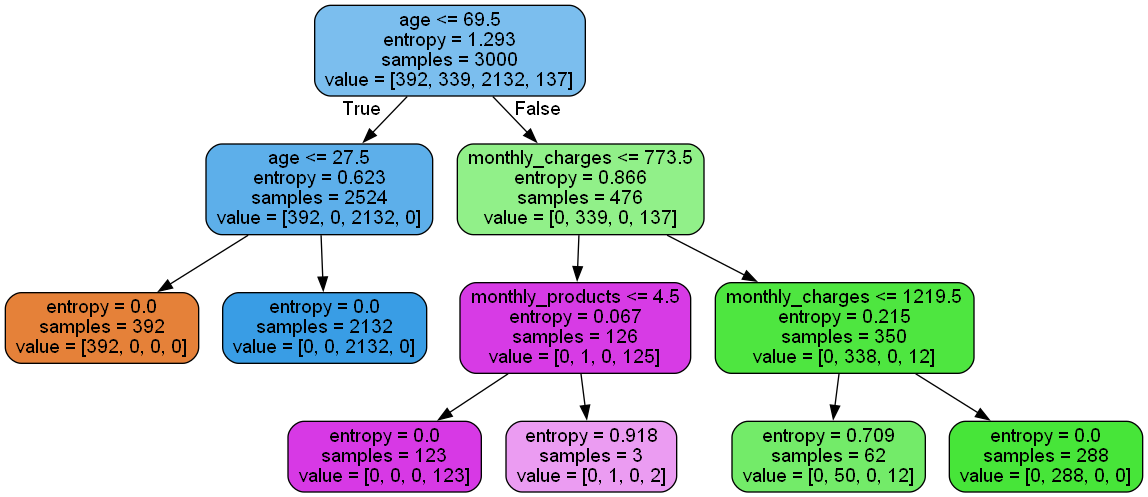
\includegraphics[width=0.95\textwidth]{tree}
\end{center}

Next, we apply this tree model to new data. In this example, I will use the test dataset. The model predicts cluster id for each customer in the test set. 

To measure the performance of the tree model, we group the customers by cluster and make a summary table that presents the count, proportion and the average of the binary target (churn or not churn).

\begin{lstlisting}[language=Python]
y_test_pred_cluster_id = tree.predict(X_test)
print('#Summary Table of the test dataset partitioned by the cluster predicted by the tree model'\n)
print(compute_target_mean_by_cluster(X_test, X.columns, y_test_pred_cluster_id, y_test))
\end{lstlisting}

\begin{lstlisting}[language=Python,numbers=none]
#Summary table of the test dataset partitioned by the cluster predicted by the tree model

            count  proportion  target(y)
cluster_id                              
0             130       0.130   0.592308
1             142       0.142   0.781690
2             673       0.673   0.049034
3              55       0.055   0.290909
\end{lstlisting}

We compare this table with the summary table for the training dataset. As we see, we have very similar average target values across clusters in the training and test sets.

\begin{lstlisting}[language=Python]
print('#Summary table of the training dataset partitioned by the cluster predicted by the random forest model\n')
print(per_cluster)
\end{lstlisting}

\begin{lstlisting}[language=Python,numbers=none]
#Summary table of the training dataset partitioned by the cluster predicted by the random forest model

            count  proportion  target(y)  target(y_hat)
cluster_id                                             
0             392    0.130667   0.599490       0.583819
1             339    0.113000   0.787611       0.723926
2            2132    0.710667   0.050188       0.115921
3             137    0.045667   0.102190       0.265285
\end{lstlisting}

\subsection{Tuning parameters}
There are several tuning parameters to consider in the process. Here, I take up two most important parameters.

\subsubsection{Cutoff point in the dendrogram}
In the example, we cut the dendrogram at the distance of 0.6, which resulted in four clusters. However, we could also choose some other cutoff points. For example, if we cut the tree at 0.45, we get six clusters as shown below. The granularity of clustering has increased. Clusters 3 and 4 in this new clustering made up a single cluster in the previous clustering, but now two separate clusters. The color indicates that the customers in Cluster 3 and 4 have different churn probabilities on average. The same applies to Cluster 1 and 5 in this new clustering although the difference in the average churn probability is less. The below is a new summary table.

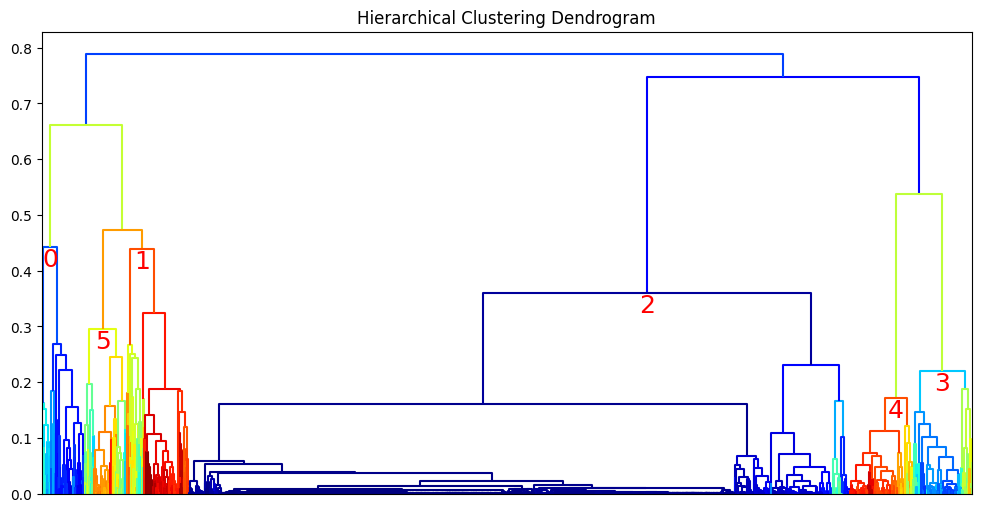
\includegraphics[width=1\textwidth]{dendrogram_depth3_colored_thres045}

\begin{lstlisting}[language=Python,numbers=none]
            count  proportion  target(y)  target(y_hat)
cluster_id                                             
0             137    0.045667   0.102190       0.265285
1             202    0.067333   0.905941       0.790902
2            2132    0.710667   0.050188       0.115921
3             192    0.064000   0.322917       0.366453
4             200    0.066667   0.865000       0.792490
5             137    0.045667   0.613139       0.625174
\end{lstlisting}

An increased granularity of clustering may increase the precision of your actions to the desired target group of customers. But at the same time, the number of resulting clusters may make the cluster management more difficult. So, you need to determine the optimal balance in the trade-off between granularity and complexity.

\subsubsection{Max depth of trees in random forest}
In the previous example, we set the max depth at 3. If we choose 5 instead, we get the following dendrogram.

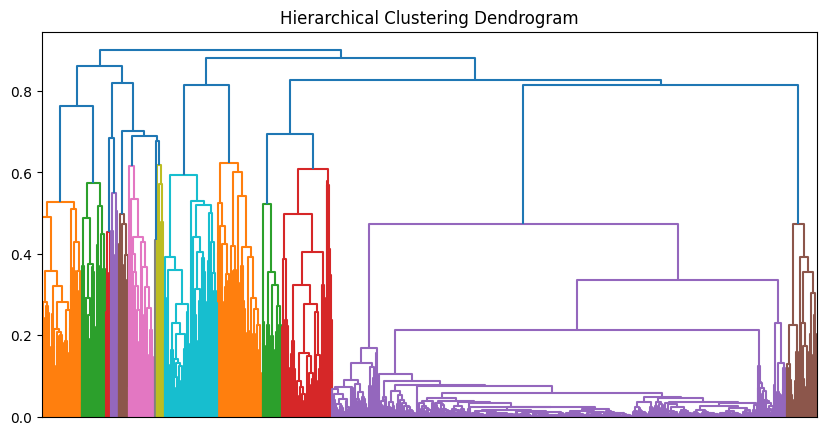
\includegraphics[width=1\textwidth]{dendrogram_depth5}

Because fewer customers end up in a single end node, the distance between customers has increased. When we cut the tree at the distance of 0.84, we get four clusters.

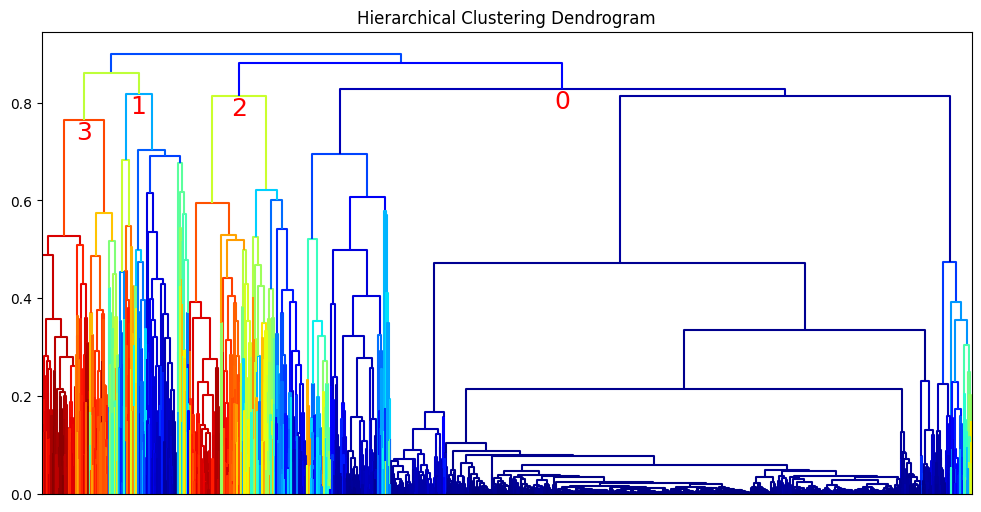
\includegraphics[width=1\textwidth]{dendrogram_depth5_colored_thres084}

Taking a look at the summary table below, we have a similar clustering as when we set the max depth to 3, in this specific example. You may have more different clustering when you choose different max depth in other cases, depending on the underlying structure in the data. 

\begin{lstlisting}[language=Python,numbers=none] 
#Summary table of the training dataset when the max depth is set to 5.

            count  proportion  target(y)  target(y_hat)
cluster_id                                             
0            2145    0.715000   0.049883       0.121736
1             226    0.075333   0.278761       0.339741
2             379    0.126333   0.620053       0.603539
3             250    0.083333   0.872000       0.814531
\end{lstlisting}

\begin{lstlisting}[language=Python,numbers=none] 
#Summary table of the training dataset when the max depth is set to 3.

            count  proportion  target(y)  target(y_hat)
cluster_id                                             
0             392    0.130667   0.599490       0.583819
1             339    0.113000   0.787611       0.723926
2            2132    0.710667   0.050188       0.115921
3             137    0.045667   0.102190       0.265285
\end{lstlisting}

\subsection{Comparison to K-means}
Finally, I present the result from a K-means clustering for comparison.

\begin{lstlisting}[language=Python] 
from sklearn.preprocessing import StandardScaler
from sklearn.cluster import KMeans

sc = StandardScaler()
X_train_std = sc.fit_transform(X_train)

km = KMeans(n_clusters=4,
            init='k-means++',
            n_init=10,
            max_iter=300, random_state=0)
y_km = km.fit_predict(X_train_std)

pd_cluster = pd.DataFrame(X_train, columns=X.columns).copy()
pd_cluster['y'] = y
pd_cluster['cluster_id'] = y_km
mean_by_cluster = pd_cluster.groupby('cluster_id')['y'].agg(['count', 'mean'])
mean_by_cluster['proportion'] = mean_by_cluster['count'] / mean_by_cluster['count'].sum()
mean_by_cluster = mean_by_cluster.sort_index()
mean_by_cluster.columns = ['count', 'target', 'proportion']
print(mean_by_cluster[['count', 'proportion', 'target']])
\end{lstlisting}

\begin{lstlisting}[language=Python] 
            count  proportion    target
cluster_id                             
0             641    0.213667  0.354134
1             816    0.272000  0.078431
2             814    0.271333  0.110565
3             729    0.243000  0.331962
\end{lstlisting}


% All content is planned to be released at https://github.com/yoshisatose/suclu
\end{document}

